\section{Exercise 10}
The forced system equation of the pendulum is given by
\begin{equation}
	ml^2\ddot{\theta} + bl\dot{\theta} + mgl\sin\theta = \tau
	\label{eq:clEq}
\end{equation}
For the PD-controller, the actuator torque will be 
\begin{equation*}
	\tau = K_p\left(\pi - \theta\right) - K_d\left(\dot{\theta}\right)
\end{equation*}
Substituting the actuator torque in \eqref{eq:clEq}, we get
\begin{equation*}
	\ddot{\theta} + \left(\frac{bl + K_d}{ml^2}\right)\dot{\theta} + \frac{mgl\sin\theta + K_p\left(\theta - \pi\right)}{ml^2} = 0
\end{equation*}

\subsection{LaSalle's Invariance Principle}
Consider an energy function $V\left(\bm{x}\right)$ of the system which is radially unbounded and positive definite. Consider a subspace $\Omega$ where $\dot{V}\left(x\right) \leq 0$. If the initial state $\bm{x}_0$ lies in this subspace, then it converges to the invariant set $S \subset \Omega$ where $\dot{V}\left(x\right) = 0$. If the set $S$ contains only the equilibrium point $\bm{x}_E$, then $\bm{x}_E$ is globally asymptotically periodic.
\subsection{Proving Asymptotic Stability}
Let the total energy of the system be the energy function candidate. Assume the lower equilibrium point $\left(0,0\right)$ is the datum. Consider $\bm{x} = \left(\theta \text{ } \dot{\theta}\right)\trans$
\begin{align*}
	V\left(\bm{x}\right) &= \frac{1}{2}ml^2\dot{\theta}^2 + mgl\left(1 - \cos\theta\right)\\
	\lim_{\|\bm{x}\|\to\infty} V\left(\bm{x}\right) &= \infty & \text{Radially Unbounded}\\
	V &> 0 & \text{Positive Definite}\\
	\dot{V} &= \left(\tau - bl\dot{\theta}\right)\dot{\theta}
\end{align*}
If $\tau = bl\dot{\theta} - k\dot{\theta}$ with $k > 0$
\begin{align*}
	\dot{V} &= -k\dot{\theta}^2 \leq 0 &\text{Semi-definite negative}\\
	\dot{V} &= 0 \Leftrightarrow \dot{\theta} = 0
\end{align*}
Hence, only the two equilibrium points $\left(0,0\right)$ and $\left(\pi,0\right)$ correspond to the invariant set which means $\left(\pi,0\right)$ is asymptotically globally stable in the presence of an actuation input.

\subsection{PD Controller Response}
The PD controller along with the euler integrator has been implemented in \emph{eulerIntegrator.py} and \emph{PD\textunderscore Pendulum.py},
The PD controller parameters are set as $K_p = 20$ and $K_d = 1$.
\begin{figure}[h!]
	\centering
	\scalebox{0.6}{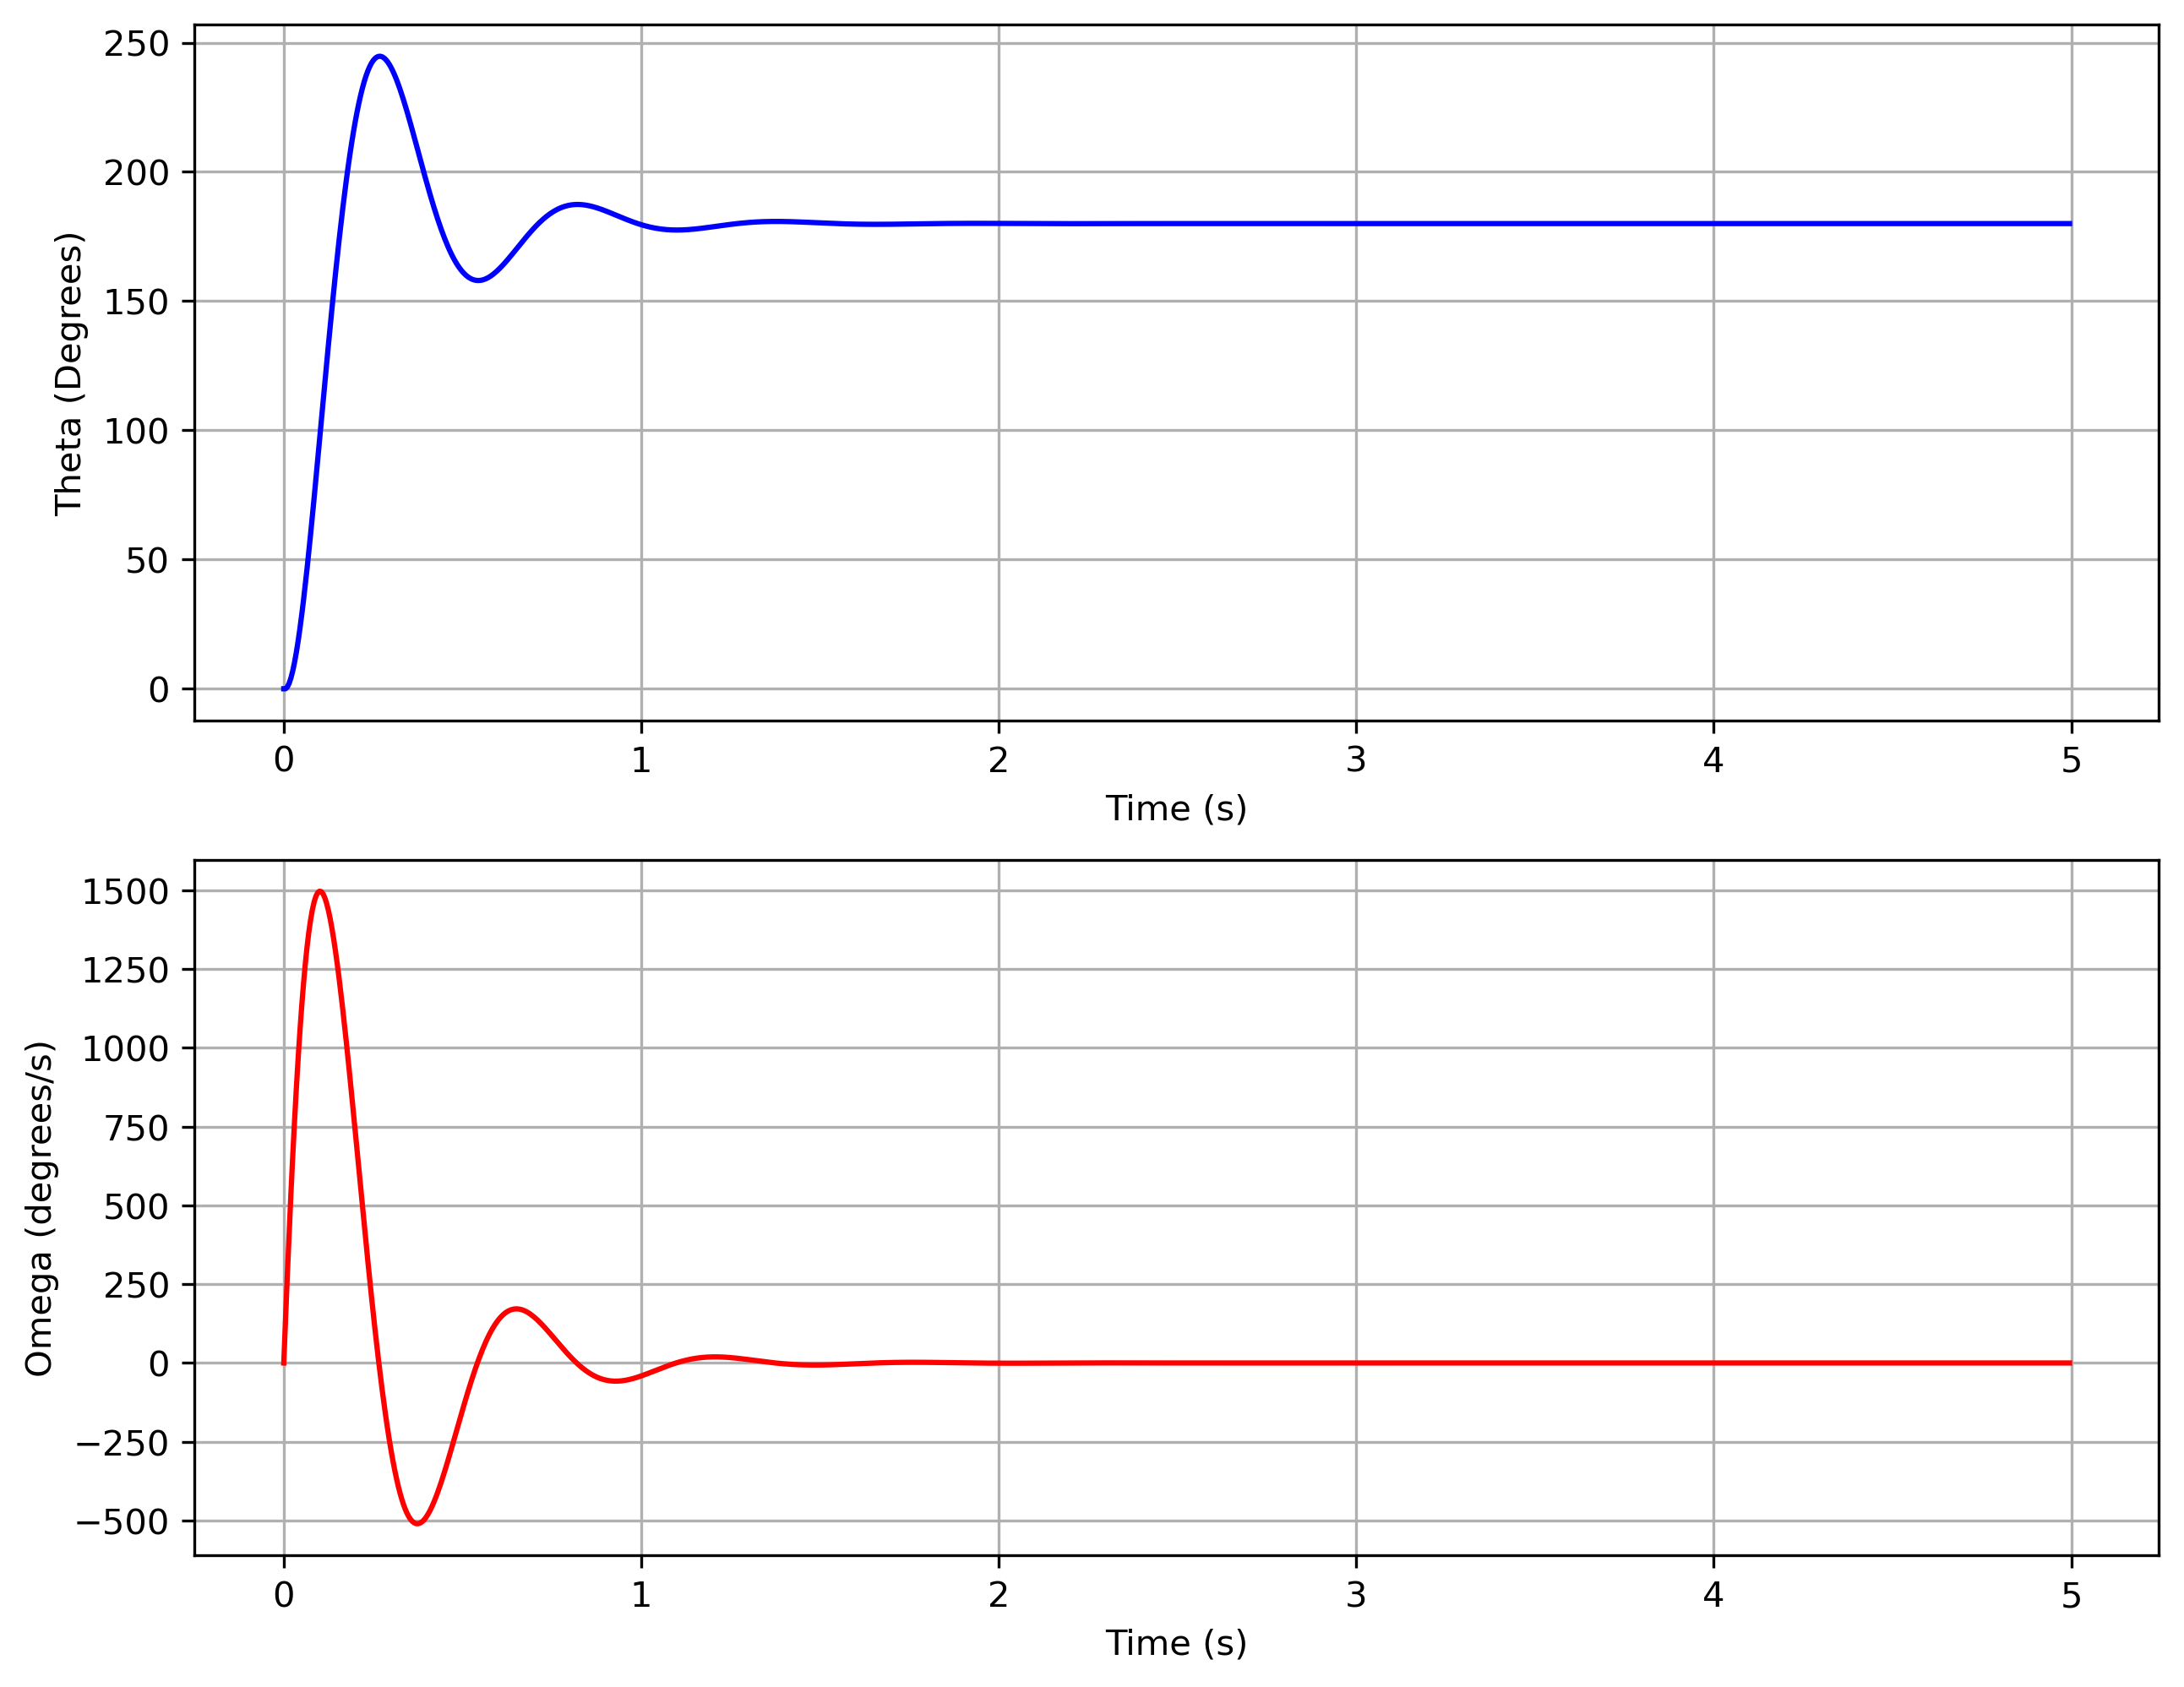
\includegraphics{images/ResponsePD_woLimit}}
	\caption{Closed-Loop System Response of PD Controller}
	\label{fig:resPD_woLimit}
\end{figure}
\begin{figure}[h!]
	\centering
	\scalebox{0.75}{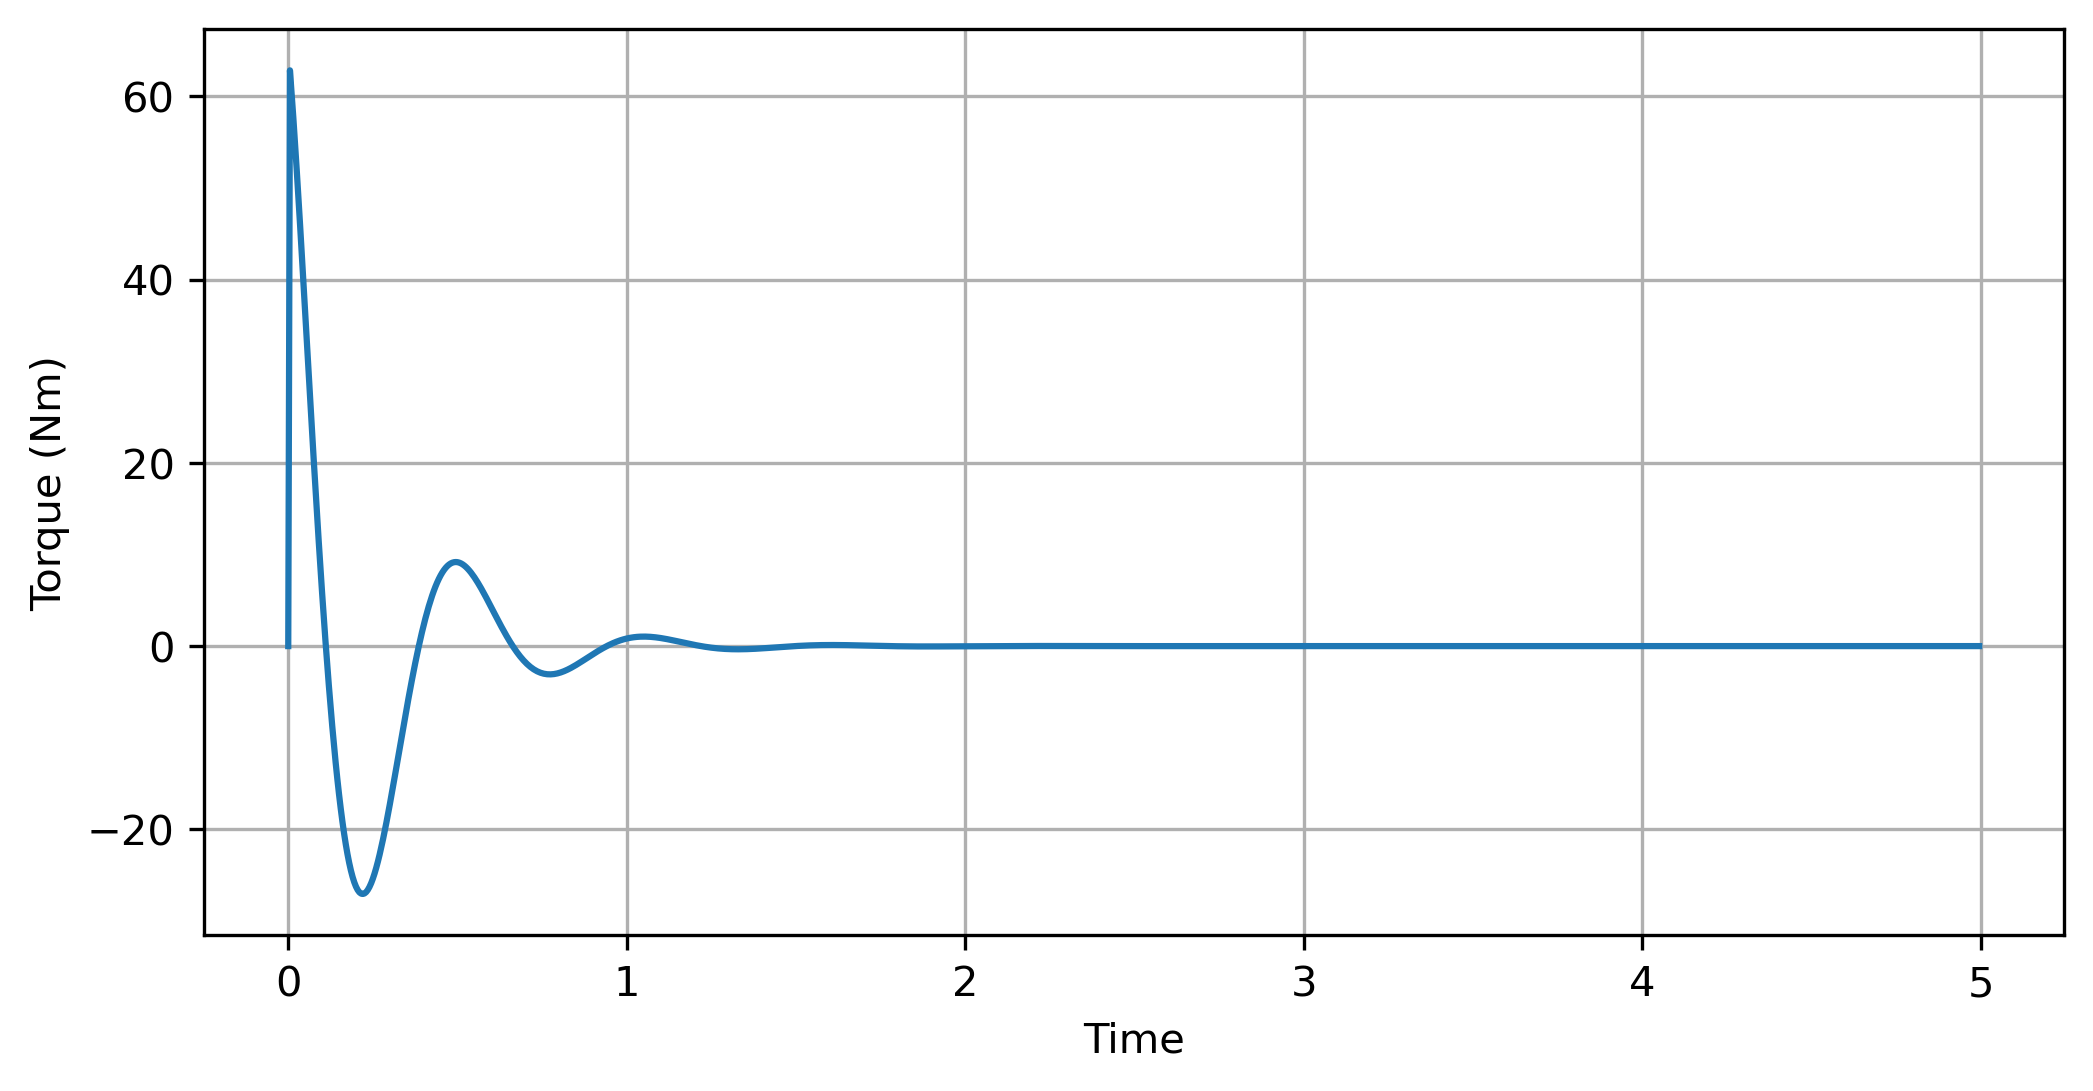
\includegraphics{images/ActuatorTorquePD_woLimit}}
	\caption{Actuator Torque (PD Controller)}
	\label{fig:actPD_woLimit}
\end{figure}

\figref{fig:resPD_woLimit} and \figref{fig:actPD_woLimit} illustrate the acceptable behaviour of the implemented PD Controller considering there are no actuator limits.

\subsection{PD Controller Response with actuator limits}
For the same controller parameters, a hard limit of $\tau_{\text{max}} = 1 Nm$ is implemented on the PD Controller.

\begin{figure}[h!]
	\centering
	\scalebox{0.6}{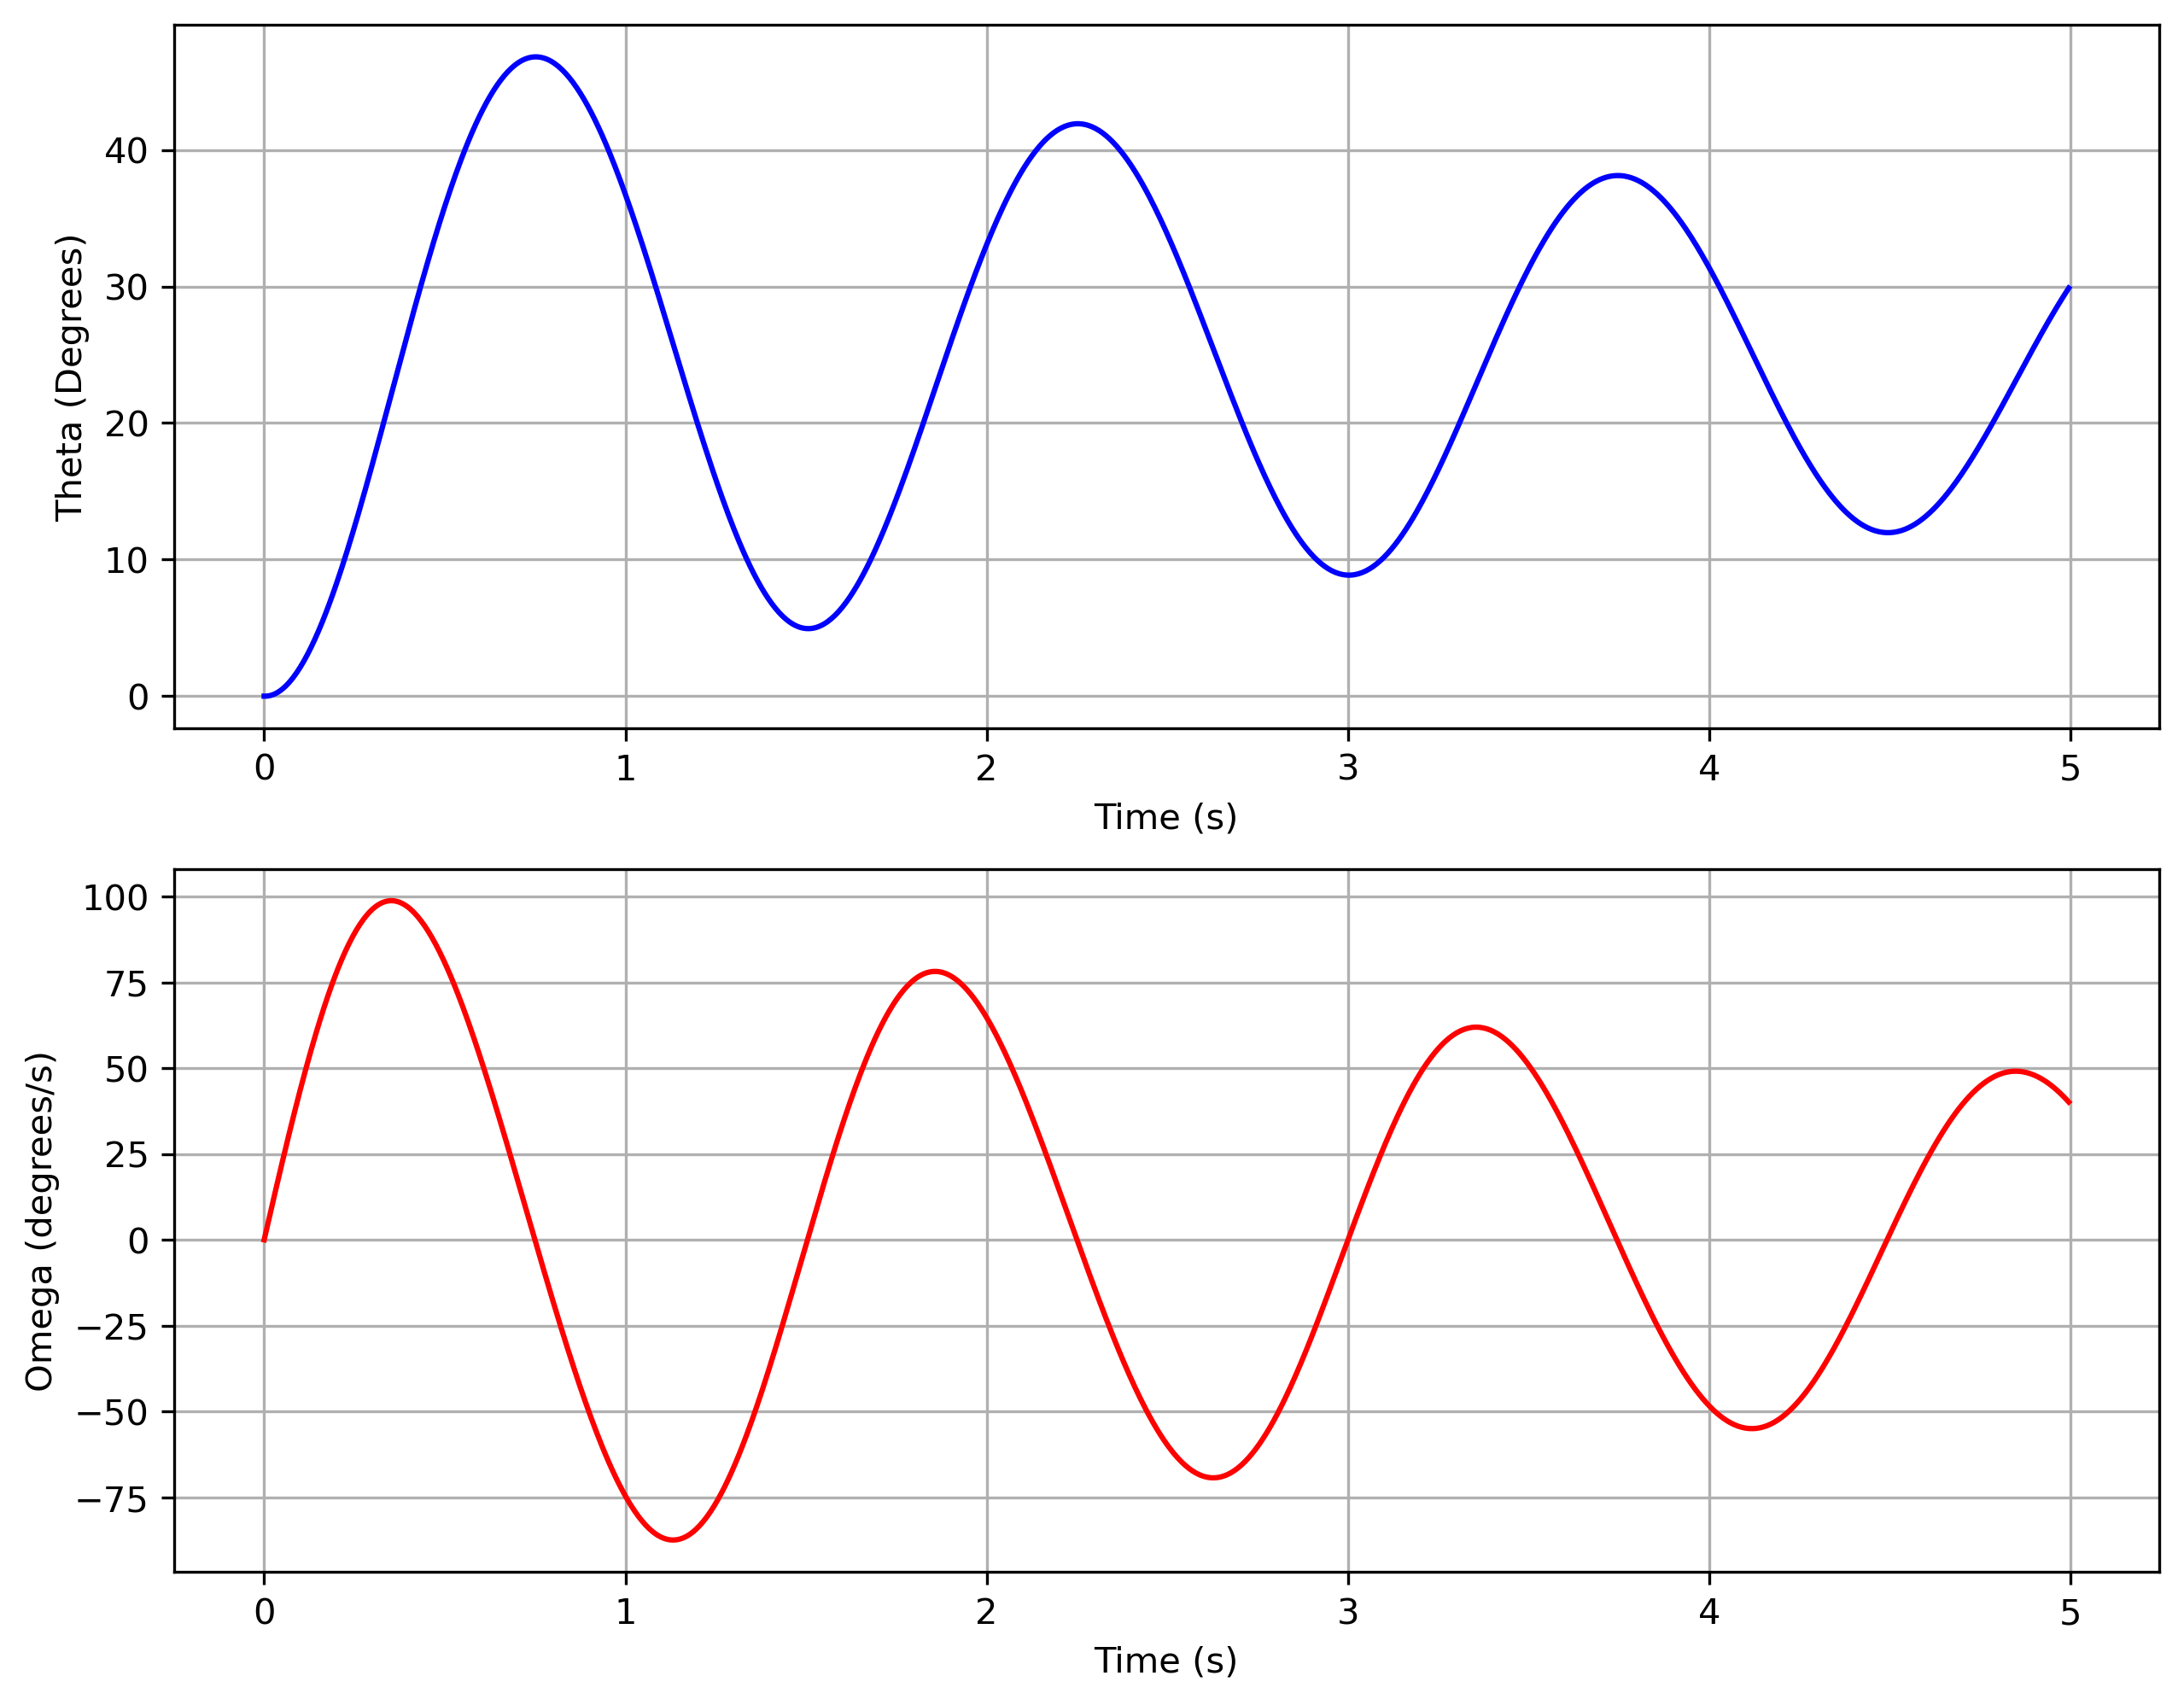
\includegraphics{images/ResponsePD_wLimit}}
	\caption{Closed-Loop System Response of PD Controller with actuator limit}
	\label{fig:resPD_wLimit}
\end{figure}
\begin{figure}[h!]
	\centering
	\scalebox{0.75}{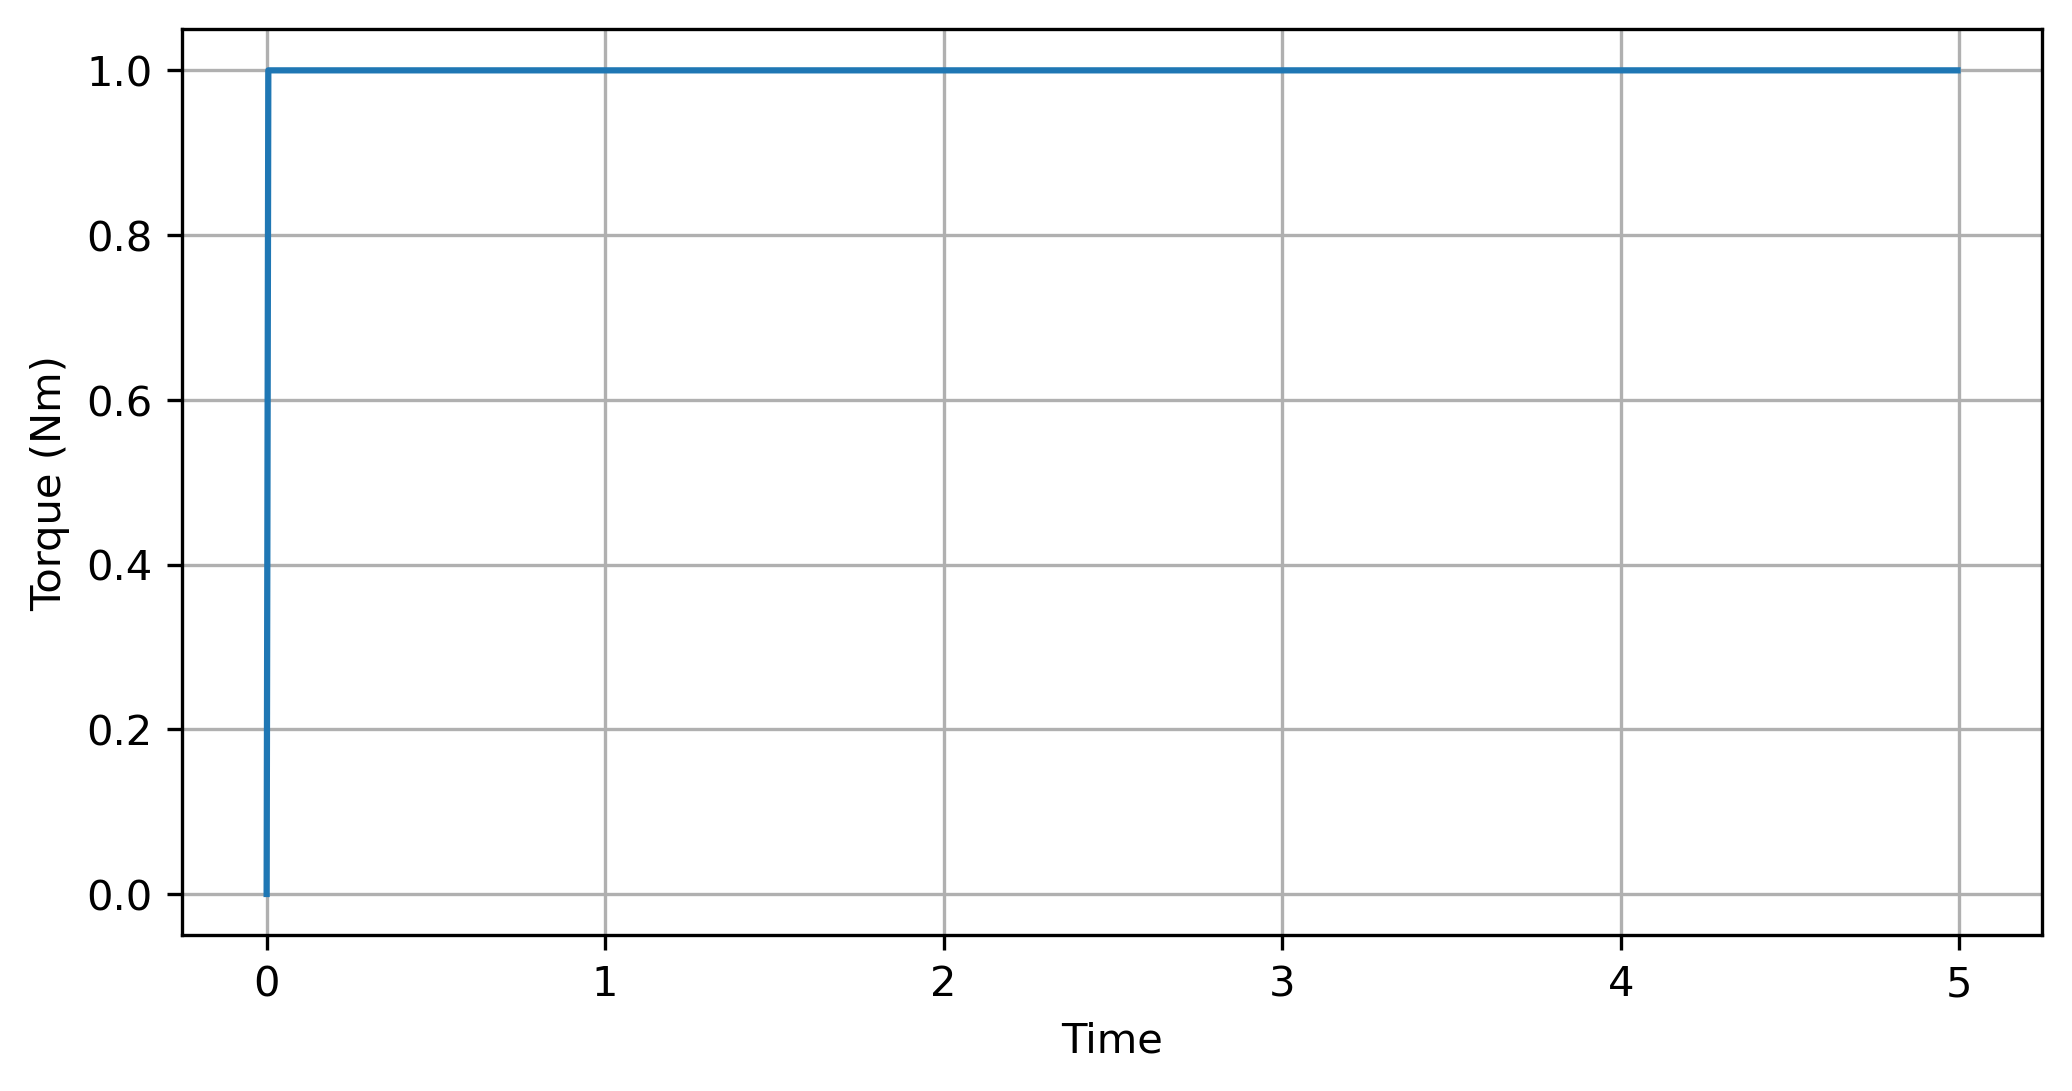
\includegraphics{images/ActuatorTorquePD_wLimit}}
	\caption{Actuator Torque (PD Controller with actuator limit)}
	\label{fig:actPD_wLimit}
\end{figure}

\figref{fig:resPD_wLimit} clearly shows that the implemented PD controller fails in presence of the actuator constraint. A possible reason for a PD controller failing to work in presence of a actuator limit (or requiring so much actuation effort in the first place) maybe due to the fact that a PD controller is essentially a linear controller, i.e. designed for a linear system, whereas the swing-up motion falls under the non-linear behaviour of the pendulum. This means that the PD controller may be more effective in balancing the pendulum around the equilibrium points (around which the system can be linearized), rather than bringing the pendulum from the downright to upright position.

\subsection{Energy-based Controller for Swing-Up}
The idea behind the control objective is to add energy to the pendulum until the desired energy is achieved i.e. the control set-point is not the angle and angular velocity, rather the energy of the pendulum at the upper equilibrium point. Assuming the potential energy datum to be at the lower equilibrium point,
\begin{align*}
	E_{\text{des}} &= 2mgl\\
	E_{\text{act}} &= \frac{1}{2}ml^2\dot{\theta}^2 + mgl\left(1 - \cos\theta\right)
\end{align*}
The actuator effort is then given by
\begin{equation*}
	\tau = K\left(E_{\text{des}} - E_{\text{act}}\right)
\end{equation*}
In order to ensure the direction of the input torque is in the current direction, the direction of $\dot{\theta}$ is monitored such that
\begin{equation*}
	\tau = K\left(E_{\text{des}} - E_{\text{act}}\right)\text{sgn}\left(\dot{\theta}\right)
\end{equation*}
Limiting the torque within $\left[-\tau_{\text{max}},\tau_{\text{max}}\right]$ gives us the final form of the actuator effort
\begin{equation*}
	\tau = \text{sat}\left(K\left(E_{\text{des}} - E_{\text{act}}\right)\text{sgn}\left(\dot{\theta}\right),\tau_{\text{max}}\right)
\end{equation*}
For the closed-loop response $K = 10$

\begin{figure}[h!]
	\centering
	\scalebox{0.6}{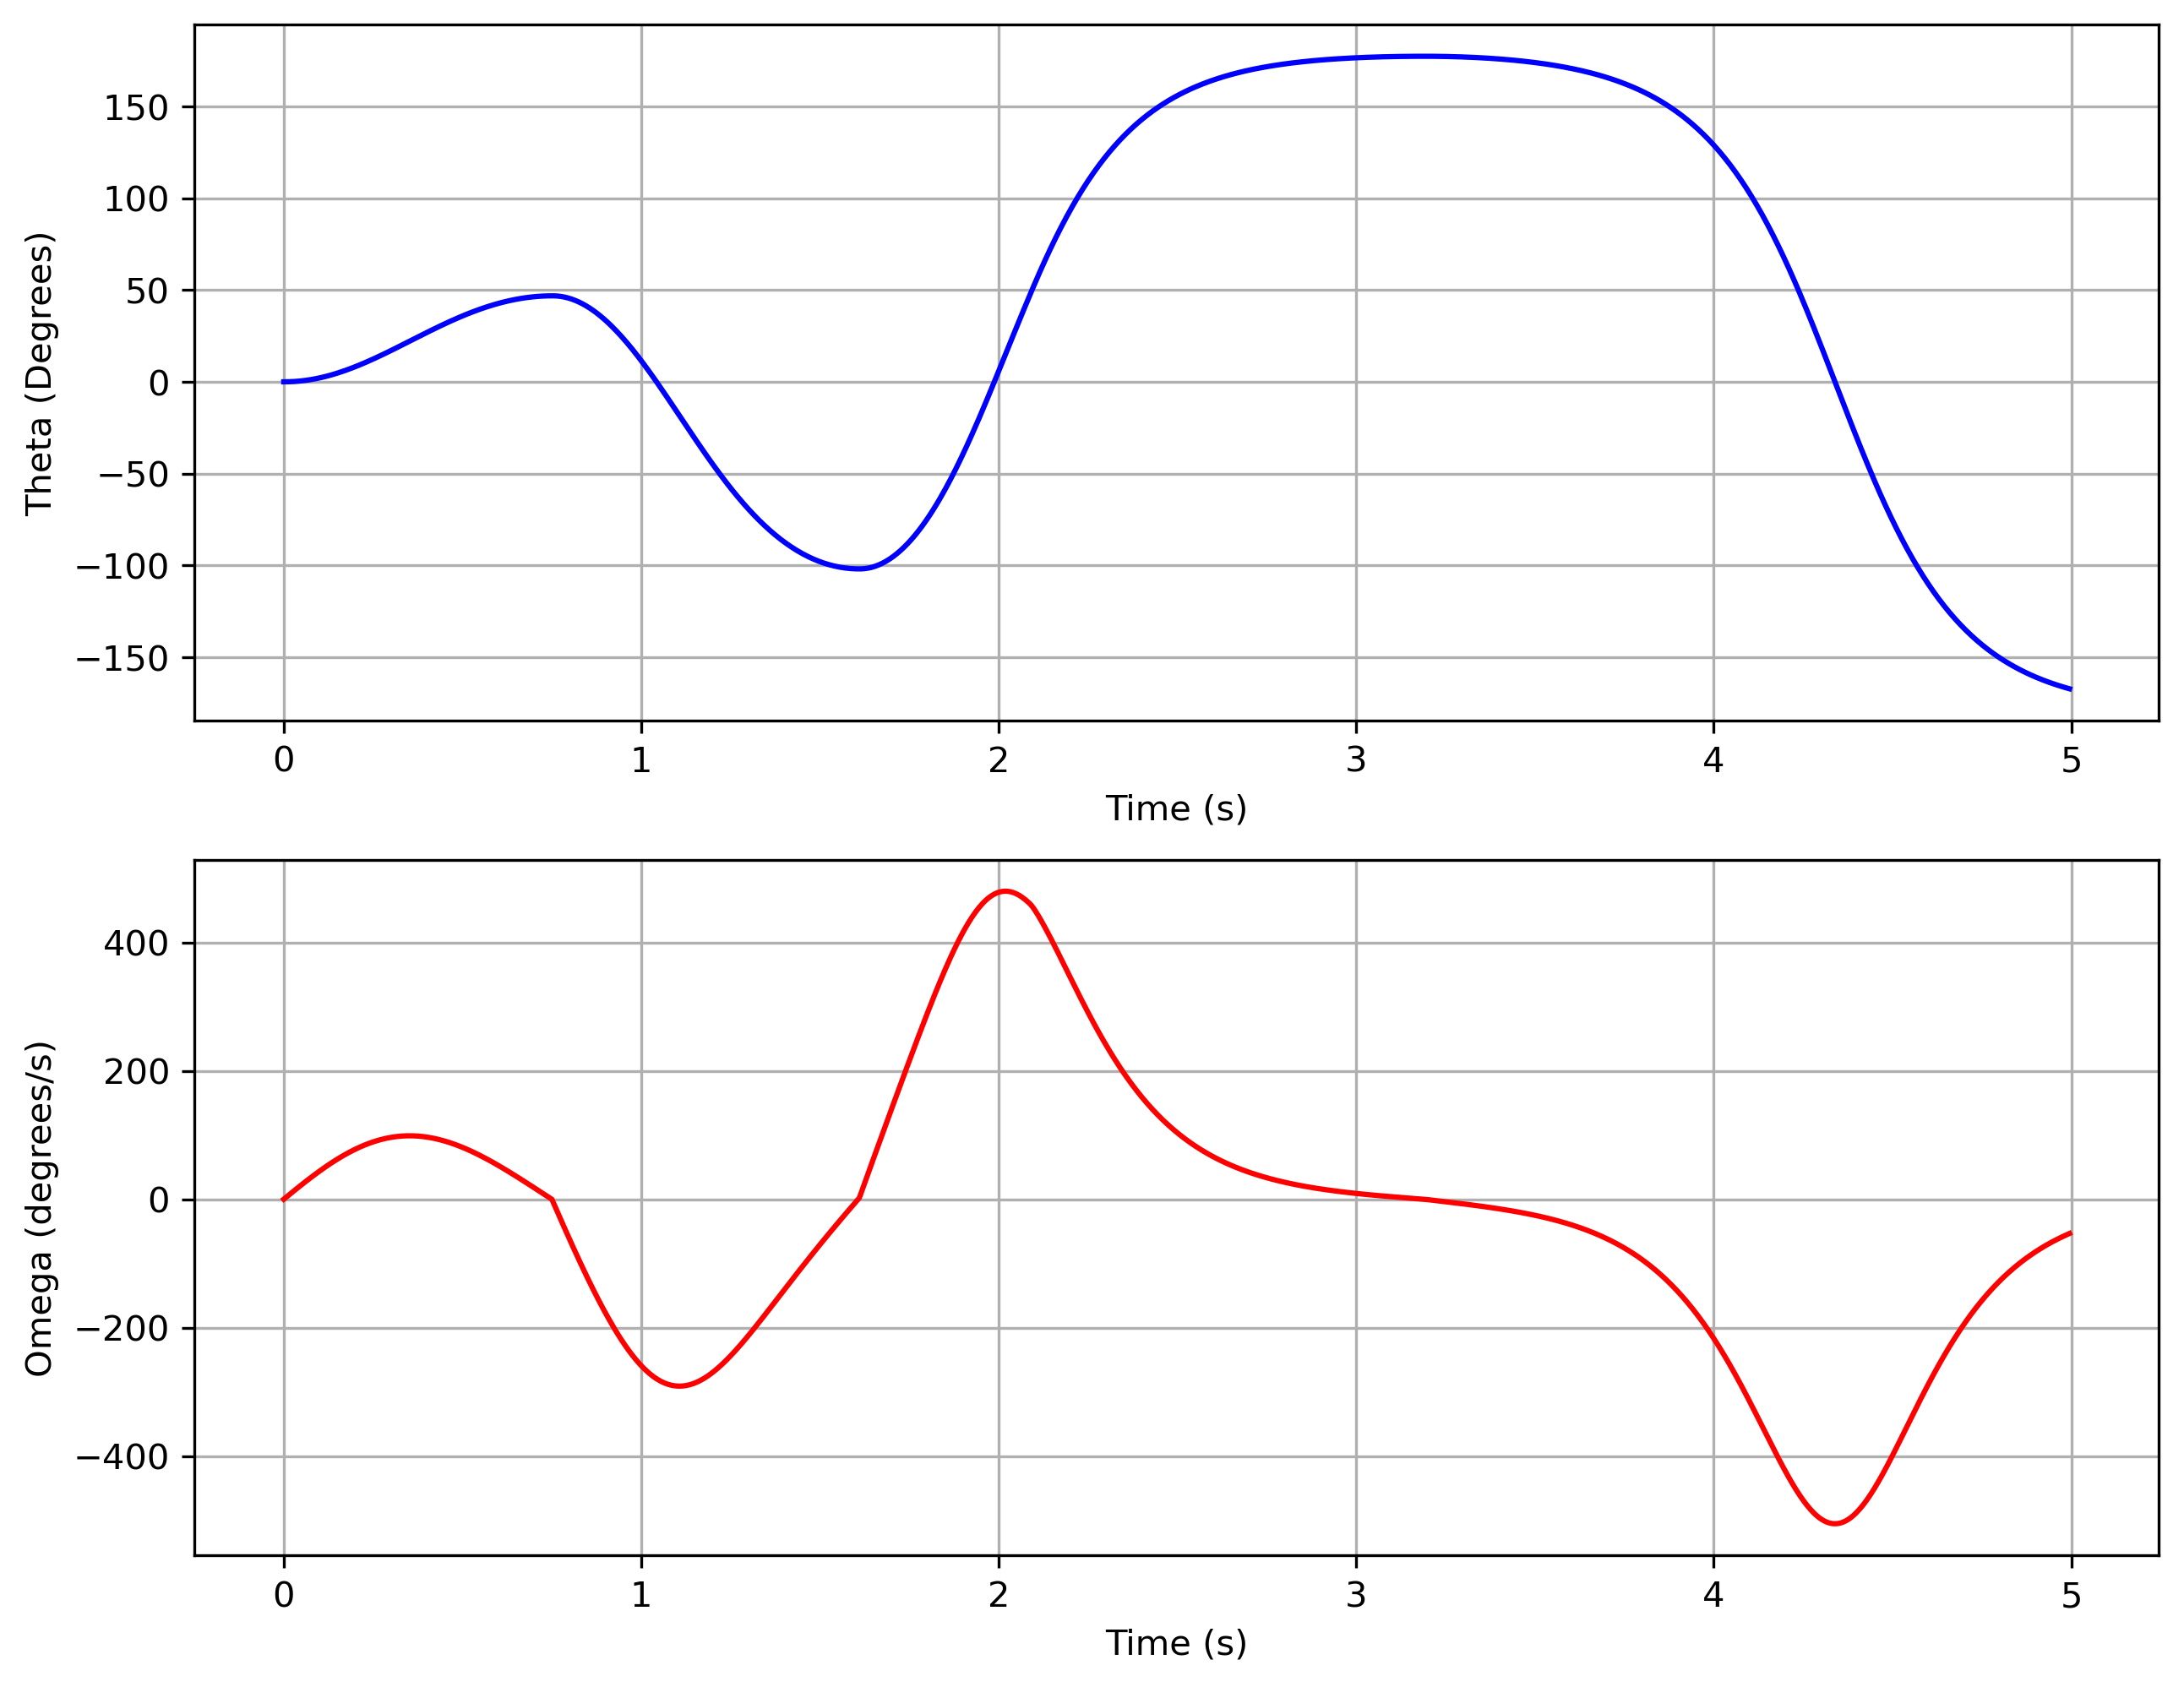
\includegraphics{images/ResponseEnergy}}
	\caption{Closed-Loop System Response of Energy based controller for swing-up}
	\label{fig:resEnergy}
\end{figure}
\begin{figure}[h!]
	\centering
	\scalebox{0.75}{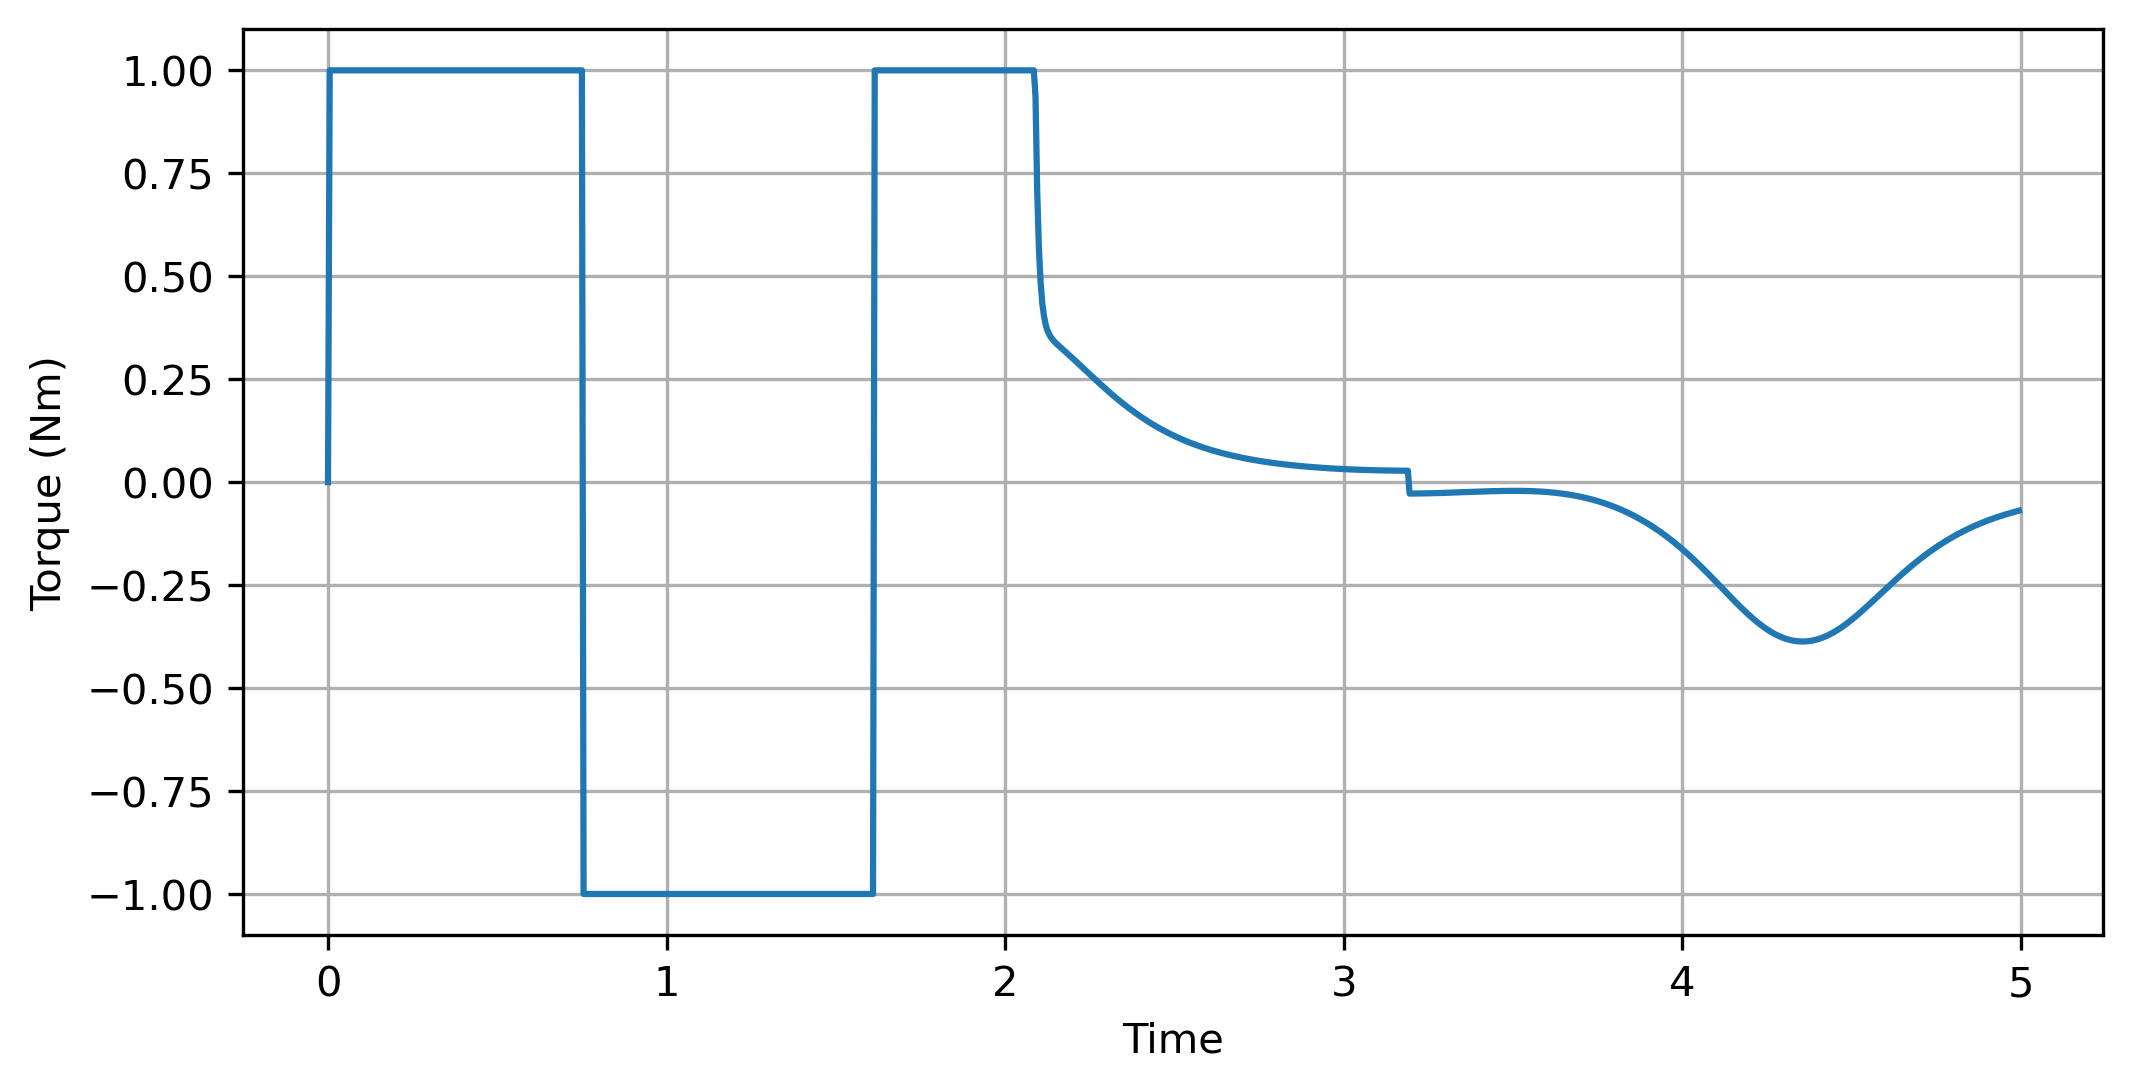
\includegraphics{images/ActuatorTorqueEnergy}}
	\caption{Actuator Torque (Energy based controller with actuator limit)}
	\label{fig:actEnergy}
\end{figure}
\figref{fig:resEnergy} illusrates that while the desired setpoint is reached (a peak of about $177$ degrees is reached) at about three seconds, the position is not maintained. On the other hand, \figref{fig:actEnergy} proves that the energy-based controller performs while maintaining the actuator limits. Furthermore it is observed for double the simulation time that the controller response essentially is cyclic i.e. it reaches the upper equilibrium point, then returns back to it from the other side ($-180$ degrees) and then the cycle continues. 

The performance may be improved by having a linear quadratic regulator take-over the energy controller when the pendulum approaches the upper equilibrium point. This is advantageous since the system can be linearized as it approaches the upper equilibrium point and the actuator limit can also be maintained since the LQR minimizes actuation energy as well.
